\documentclass{beamer}

\usepackage{../cppenv, ../recdefs}

\usepackage{drawstack}

\usetheme{Berkeley}

\title{Exception Safety and Exception Handling}
\author{GKxx}
\date{\today}

\begin{document}

\begin{frame}
    \maketitle
\end{frame}

\begin{frame}{Contents}
    \tableofcontents
\end{frame}

\section{Things Tend to Go Wrong}

\begin{frame}[fragile]{\ttt{strcpy}}
    You are asked to write a \ttt{strcpy} function...
    \begin{cpp}
void strcpy(char *dest, const char *source) {
  while (*source)
    *dest++ = *source++;
  *dest = '\0';
}
    \end{cpp}
    \pause
    In reality, things may go wrong:
    \begin{itemize}
        \item Null pointers?
        \item Buffer overflow?
    \end{itemize}
    We may not be able to detect buffer overflow.
\end{frame}

\begin{frame}[fragile]{Which is Better?}
    \begin{columns}
        \begin{column}{0.5\textwidth}
            1. Terminate the program on failure and report the error.
            \begin{cpp}
void strcpy(char *dest,
    const char *source) {
  if (!dest || !source) {
    std::cerr << "Invalid arguments for strcpy.\n";
    exit(1);
  }
  while (*source)
    *dest++ = *source++;
  *dest = '\0';
}
            \end{cpp}
        \end{column}
        \begin{column}{0.5\textwidth}
            2. Return false on failure:
            \begin{cpp}
bool strcpy(char *dest,
    const char *source) {
  if (!dest || !source)
    return false;
  while (*source)
    *dest++ = *source++;
  *dest = '\0';
  return true;
}
            \end{cpp}
            3. Be silent and just let the user ensure that the arguments are valid.
        \end{column}
    \end{columns}
\end{frame}

\section{Exception in C++}

\subsection{\ttt{throw}}

\begin{frame}[fragile]{Throwing an Exception}
    \begin{cpp}
void strcpy(char *dest, const char *source) {
  if (!dest || !source)
    throw std::invalid_argument("Null pointers passed to strcpy.");
  while (*source)
    *dest++ = *source++;
  *dest = '\0';
}
    \end{cpp}
\end{frame}

\begin{frame}{Standard Exceptions}
    \begin{center}
        \includegraphics[width=0.9\textwidth]{img/ExceptionClasses.jpg}
    \end{center}
    \begin{itemize}
        \item \ttt{logic\_error}, \ttt{runtime\_error} and their subclasses are defined in \ttt{<stdexcept>}.
    \end{itemize}
\end{frame}

\begin{frame}{Standard Exceptions}
    \begin{itemize}
        \item The normal \bluett{new} and \bluett{new}\ttt{[]} operators throw \ttt{std::bad\_alloc} when running out of memory.
        \item \bluett{dynamic\_cast} for references throws \ttt{std::bad\_cast} when the casting fails.
        \begin{itemize}
            \item \bluett{dynamic\_cast} for pointers does not throw. It returns \bluett{nullptr} on failure.
        \end{itemize}
        \pause
        \item \ttt{std::system\_error} is thrown in many cases, especially in functions that interface with \blue{OS facilities}, e.g. the constructor of \ttt{std::thread}.
        \item \ttt{<chrono>} defines \ttt{std::nonexistent\_local\_time} and \ttt{std::ambiguous\_local\_time}.
    \end{itemize}
\end{frame}

\begin{frame}[fragile]{Standard Exceptions}
    \ttt{operator[]} for STL containers does not check boundaries, but \ttt{at()} does.
    \begin{cpp}
std::vector<int> v;
v.at(0) = 42; // Throws std::out_of_range.
v[0] = 42; // Does not throw, but probably causes a segmentation fault.
    \end{cpp}
    We will see that exceptions \bluett{throw}n could be \bluett{catch}ed and handled.
\end{frame}

\begin{frame}[fragile]{Standard Exceptions}
    Let our \ttt{Array} do the same thing?
    \begin{cpp}
template <typename T>
class Array {
 public:
  T &at(std::size_t n) {
    if (n >= m_size)
      throw std::out_of_range("Array subscript out of range.");
    return m_data[n];
  }
  const T &at(std::size_t n) const {
    // ...
  }
  // ...
};
    \end{cpp}
\end{frame}

\begin{frame}[fragile]{Call Stack Unwinding}
    \begin{columns}
        \begin{column}{0.5\textwidth}
            \begin{cpp}
void func(int n) {
  int x = 42;
  int *p = new int[n];
  // ...
}
int main() {
  int size = 100;
  func(size);
  // ...
}
            \end{cpp}
        \end{column}
        \begin{column}{0.5\textwidth}
            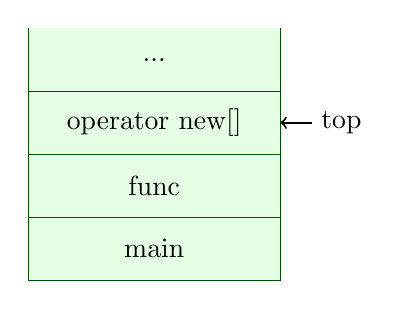
\begin{tikzpicture}[scale=0.8]
                \stacktop{}
                \cell{\bluett{operator new}\ttt{[]}}\cellptr{top}
                \cell{\ttt{func}}
                \cell{\ttt{main}}
            \end{tikzpicture}
        \end{column}
    \end{columns}
    Suppose \bluett{operator new}\ttt{[]} encounters shortage of memory...
\end{frame}

\subsection{\ttt{try}-\ttt{catch}}

\end{document}